\documentclass[article,12pt,onesidea,4paper,english,brazil]{abntex2}

\usepackage{lmodern, indentfirst, nomencl, color, graphicx, microtype, lipsum}			
\usepackage[T1]{fontenc}		
\usepackage[utf8]{inputenc}
\usepackage{textcomp}		

\setlrmarginsandblock{2cm}{2cm}{*}
\setulmarginsandblock{2cm}{2cm}{*}
\checkandfixthelayout

\setlength{\parindent}{1.3cm}
\setlength{\parskip}{0.2cm}

\SingleSpacing

\begin{document}
	
	\selectlanguage{brazil}
	
	\frenchspacing 
	
	\begin{center}
		\LARGE ESTUDO SOBRE EVASÃO NOS CURSOS À DISTÂNCIA E PRESENCIAL DO IFRO- CÂMPUS PORTO VELHO ZONA NORTE
		
		\normalsize
		Daiana Cavalcante Gomes\footnote{Bolsista PIBIC, daianasabina@gmail.com.br, Campus Porto Velho Zona Norte} 
		Maria Beatriz Souza Pereira\footnote{Bolsista PIBIC, mbe.pereira@gmail.com.br, Campus Porto Velho Zona Norte.} \\
		Lady Day Pereira de Souza\footnote{Orientadora, lady.souza@ifro.edu.br, Campus Porto Velho ZonaNorte..} 
	Dinalva Barbosa da Silva Fernandes\footnote{Coorientadora, dinalva.fernandes@ifro.edu.br, Campus Porto Velho Zona Norte.} 
	\end{center}
	
	% resumo em português
	\begin{resumoumacoluna}
	Este estudo tem objetivo de conhecer o perfil dos alunos que compõem o percentual de evasão nos cursos oferecidos pelo IFRO - Campus Porto Velho Zona Norte no período de 2013 a 2015. Para que possamos identificar os motivos da desistência dos alunos, através de entrevistas, tem sido aplicado um questionário com 26 perguntas abertas e fechadas. A parte presencial da pesquisa já foi concluída, quanto aos alunos da modalidade EaD, considerando que são mais numerosos, a pesquisa ainda está em andamento. Assim, ao final da pesquisa e com base nos dados obtidos, espera-se poder contribuir com a instituição para que seja capaz de promover mudanças estratégicas para estimular a permanência e o êxito dosestudantes.
	
	
		
		\vspace{\onelineskip}
		
		\noindent
		\textbf{Palavras-chave}:Evasão Escolar. Educação a Distância. Instituto Federal de Rondônia.
	\end{resumoumacoluna}
	
	\section*{Introdução}
	
	Este projeto visa conhecer o perfil dos alunos responsáveis pelo crescente percentual da evasão nos cursos oferecidos pelo Campus Porto Velho Zona Norte - IFRO. O ensino a distância ofertado pelo IFRO tem auxiliado na formação de vários profissionais atuantes no mercado de trabalho, a prova disso são as parcerias firmadas com as prefeituras para a criação de novos polos. Neste contexto, busca- se o entendimento sobre os principais aspectos e fatores que envolvem a evasão nos cursos, bem como a identificação das principais causas da evasão escolar,com intuito de, ao dimensionar o quadro atual em relação à evasão, propor medidas de combate à mesma.
	
	\section*{Material e Método}
	
	Para que possamos identificar os motivos da desistência dos alunos, através de entrevistas, tem sido aplicado um questionário com 26 perguntas abertas e fechadas. A parte presencial da pesquisa já foi concluída, quanto aos alunos da modalidade EaD, considerando que são mais numerosos, a pesquisa ainda está em andamento.
	
	O quantitativo de alunos dos cursos presenciais foi possibilitado através do levantamento de dados nas planilhas disponibilizadas pela CRA, contendo a matrícula escolar dos alunos no primeiro período e rematrículas nos períodos seguintes. O cruzamento dessa informação resultou numa amostra de 245 alunos evadidos dos cursos presenciais. Foram realizadas, através de ligação telefônica, entrevistas aos alunos evadidos, e do total, 100 alunos atenderam as ligações, contudo, somente 80 aceitaram fazer parte da pesquisa, sendo a amostra final. O tratamento dos dados foi realizado através do software de estatística IBM SPSS 21. A seguir a demonstração dos resultados.
	
	\section*{Resultados e Discussão}
	
O estudo sobre a evasão do Campus Porto Velho Zona Norte concluiu a etapa referente ao ensino presencial, apresentando os dados referentes aos anos de 2013, 2014, e, 2015 através de gráficos. Serão expostos resultados do curso superior de Tecnologia em Gestão Pública, dos Cursos Técnicos em Informática para Internet e em Finanças Subsequentes ao Ensino Médio.

No primeiro gráfico apresentado serão demonstrados os números do curso de Tecnologia em Gestão Pública referente ao quantitativo de alunos matriculados, evadidos e os alunos que aceitaram fazer parte da pesquisa, os entrevistados:
\begin{figure}[h]
	\centering
	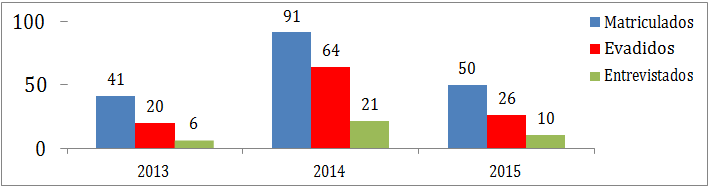
\includegraphics[width=0.5\linewidth]{pip-pg78-01}
	\caption{Evasão escolar dos alunos do curso de Gestão Pública.}
	\label{fig:pip-pg78-01}
\end{figure}

O próximo gráfico se refere ao Curso Técnico em Informática para Internet. Com dados referentes ao quantitativo de alunos matriculados, evadidos, e, os alunos que aceitaram fazer parte da pesquisa, os entrevistados:
\begin{figure}[h]
	\centering
	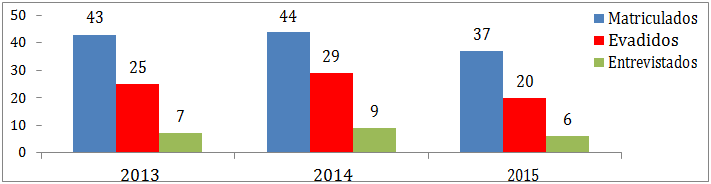
\includegraphics[width=0.5\linewidth]{pip-pg78-02}
	\caption{Evasão escolar dos alunos do curso Técnico de Informática.}
	\label{fig:pip-pg78-02}
\end{figure}

O gráfico a seguir é referente ao quantitativo de alunos do curso técnico em Finanças matriculados, evadidos, e, os que aceitaram fazer parte da pesquisa, os entrevistados.
\begin{figure}[h]
	\centering
	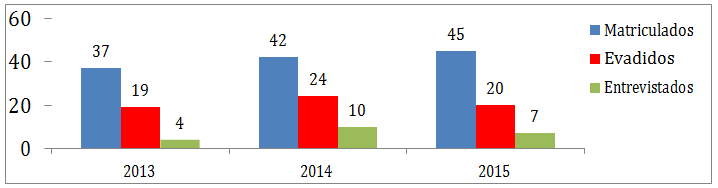
\includegraphics[width=0.5\linewidth]{pip-pg78-03}
	\caption{Evasão escolar dos alunos do curso Técnico de Finanças}
	\label{fig:pip-pg78-03}
\end{figure}


Após atender a ligação e explicada a pesquisa ao participante, e, somente com a confirmação de seu aceite, os alunos eram submetidos a um questionário. A
primeira fase continha perguntas para identificação, seguida por uma fase em que era questionado quanto à evasão do curso. Em seguida, pedíamos que mencionassem até três motivos para a evasão do curso, fato que somadas às respostas ultrapassarão cem por cento (100\%). O próximo gráfico evidencia os motivos apontados pelos alunos para o abandono dos estudos:
\begin{figure}[h]
	\centering
	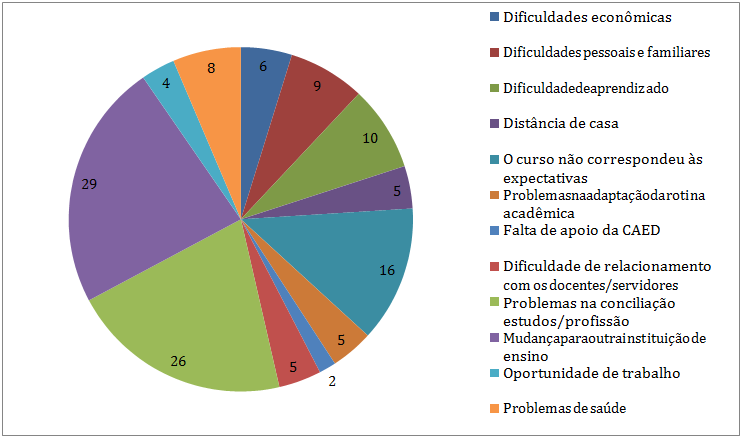
\includegraphics[width=0.7\linewidth]{pip-pg78-04}
	\caption{Justificativas dos alunos como motivos para a evasão.}
	\label{fig:pip-pg78-04}
\end{figure}

Os alunos foram questionados acerca de um possível reingresso ao IFRO, mas dessa vez podiam optar por apenas uma resposta. A seguir o gráfico:
\begin{figure}[h]
	\centering
	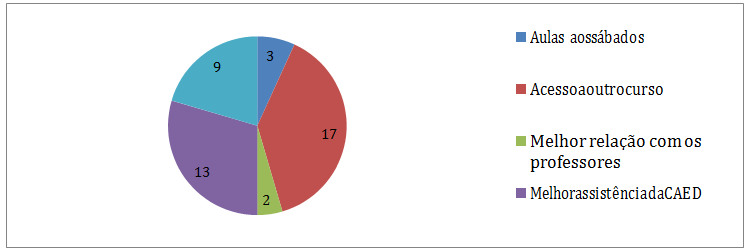
\includegraphics[width=0.7\linewidth]{pip-pg78-05}
	\caption{Razões apontadas pelos alunos para o reingresso.}
	\label{fig:pip-pg78-05}
\end{figure}	
	\section*{Conclusões}
	
Como obtivemos apenas resultados dos cursos presenciais, podemos apontar que os alunos em sua maioria afirmam que interromperam os estudos por que mudaram para outra instituição de ensino superior, ou, porque não conseguem conciliar o estudo com o trabalho, seguido por alegarem que o curso não correspondeu	às	expectativas.	Mas	quanto à possibilidade de reingresso no IFRO, surge na pesquisa como algo que consideramos positivo, ou seja, as pessoas realmente sabem que a formação profissional é necessária para melhorar a renda e reconhecem os esforços do Instituto Federal de Rondônia em promover a democratização da educação pública, gratuita e de qualidade, por meio da modalidade adistância.
	
	\section*{Instituição de Fomento}
	
	O Instituto Federal de Educação, Ciência e Tecnologia de Rondônia, Campus Porto Velho Zona Norte, possibilitou a pesquisa ao aprová-la em edital, a saber, N°31 do mês de julho do ano de 2015.
	
	
	
	\section*{Referências}
	
\noindent AGENCIA BRASIL. Jovens no Brasil trabalham mais e estudam menos, mostra relatório	da	OCDE.	2015.	Disponível	em:
<http://agenciabrasil.ebc.com.br/educacao/noticia/2015-11/editada-jovens-no-brasil-trabalham-mais-e-estudam-menos-mostra-relatorio>. Acesso em junho/ 2016

\noindent ALVES, Lucineia. Educação a distância: conceitos e história no Brasil e no mundo. Revista Brasileira de Aprendizagem Aberta e a Distância. RBAAD. 2011. Volume	10.	Disponível	em:
<http://www.abed.org.br/revistacientifica/Revista\_PDF\_Doc/2011/Artigo\_07.pdf>. Acesso em: junho/2016.

	
\end{document}